\documentclass[twoside,UTF8]{EPURapport}
\usepackage{listings}

%\renewcommand{\lstlistlistingname}{Liste des codes}
%\renewcommand{\lstlistingname}{Code}

%\addextratables{%
%	\lstlistoflistings
%}

%\swapAuthorsAndSupervisors




\thedocument{Rapport de Projet}{Batching et optimisation des trajectoires de picking dans un centre d'entreposage}{Batching et picking}

\grade{Département Informatique\\ 3\ieme{} année\\ 2008 - 2009}

\authors{%
	\category{Étudiants}{%
		\name{Shimeng ZHANG} \mail{shimeng.zhang@etu.univ-tours.fr}
		\name{Natacha MARLIO-MARETTE} \mail{natacha.marlio-marette@etu.univ-tours.fr}
	}
	\details{DI3 2012 - 2013}
}

\supervisors{%
	\category{Encadrants}{%
		\name{Ameur SOUKHAL} \mail{ameur.soukhal@univ-tours.fr}
	}
	\details{Université François-Rabelais, Tours}
}

\abstracts{Description en français}
{Mots clés français}
{Description en anglais}
{Mots clés en anglais}






\begin{document}

%%%%%%%%%%%%%%%%%%%% INTRODUCTION %%%%%%%%%%%%%%%%%%%%

\chapter{Introduction}

%%%%%%%%%%%%%%%%%%%% CHAPITRE 1 %%%%%%%%%%%%%%%%%%%%%%

\chapter{Présentation du projet}

\section{Définitions et mise en place du problème}
\subsection{Définitions}
\paragraph{}Dans cette partie, nous définirons quelques notions permettant une meilleure compréhension de ce rapport.
\begin{description}
\item[• Picking]: C'est l'opération qui consiste à prélever les articles dans la quantité demandé par la commande avant son expédition.

\item[• Cluster]: Ce terme peut être employé dans plusieurs domaines tels que les sciences, l'informatique ou bien la musique. Ici, un cluster correspond au regroupement des objets au ceint d'un ensemble.
\item[• Heuristique] : Une heuristique est une méthode de calcul qui fournit rapidement une solution réalisable. Mais cette solution n'est pas nécessairement optimale. Ce terme s'applique pour un problème d'optimisation NP-difficile.
\end{description}


\subsection{Mise en place du problème }
\paragraph{}La problématique de ce projet est de trouver l'itinéraire que doit réaliser chaque chariot au ceint d'un entrepôt. Pour ce faire nous avons réaliser un programme en C qui définit la tournée que doit effectuer le chariot. Cependant nous avions quelques contraintes à respecter (cf la section \ref{sec:Contraintes} page \pageref{sec:Contraintes}). Pour cela nous avons utiliser différents heuristiques, il faudra par la suite en effectuant des tests déterminer le meilleur.


\section{Cahier des Charges}
\subsection{Cahier des Charges}
\paragraph{}Pour répondre à la problématique de ce projet, nous devions respecter un cahier des charges. Afin de trouver, l'itinéraire qu'emprunteront les chariots, nous avons utiliser différentes méthodes(cf les sections \ref{sec:CFRS} page \pageref{sec:CFRS} et \ref{sec:RFCS} page \pageref{sec:RFCS}). Nous avons considéré pour tout ce projet qu'un unique chariot et des objets avec un poids unique. 

\paragraph{}Pour chercher l'itinéraire de notre chariot, il faut tout d'abord lui dire ce qu'il doit aller chercher dans l'entrepôt. C'est à dire lui donner un carnet de commandes. Il faut connaître la position de chaque objet dans l'entrepôt ainsi que leur poids. Ces deux éléments seront donnés avec le carnet de commandes.

\paragraph{}Après la réalisation des différents heuristiques, il faudra faire une série de test de façon à savoir lequel est le meilleur des deux. Ces tests sont expliqués dans le chapitre \ref{chap:test} page \pageref{chap:test}.

\subsection{Contraintes}
\label{sec:Contraintes}
\paragraph{}Dans ce projet, il faut tenir compte de certaines contraintes : 
\begin{itemize}
\item[•]\textbf{La capacité du chariot}: En effet, celui-ci ne peut contenir qu'une certaine quantité (un certain poids).
\item[•]\textbf{La compatibilité et incompatibilité des produits} : Il faut tenir compte de la compatibilité des produits, de façon à ce qu'aucun produits ne soient écrasé dans le chariot.
\item[•]\textbf{Zone d'exclusion mutuelle}: Il faut synchroniser les itinéraires de façon à éviter que les chariots puissent entrer en collision. 
\item[•]\textbf{La cartographie de l'entrepôt} : Celle-ci étant inconnue, il est difficile de calculer un itinéraire exact pour le chariot. Ce qui a un impact sur la distance totale que le chariot devra parcourir.
\end{itemize} 

Nous n'avons pour ce projet tenu compte uniquement de la première contrainte.

\section{Différentes méthodes de batching et picking}

Il existe différentes méthodes de batching et picking. Durant ce projet, nous avons mis en œuvre les deux premières présentées ci-dessous.

\subsection{Cluster First Root Second}
\label{sec:CFRS}

\paragraph{}La méthode \textit{Cluster First Root Second} signifie que l'on s'occupe en premier des clusters et en second de l'itinéraire. C'est à dire que l'on découpe tout d'abord la commande en cluster. On va couper la commande à chaque fois que le chariot sera plein. Et ensuite l'on définit l'itinéraire de chaque cluster. 

\subsection{Root First Cluster Second}
\label{sec:RFCS}
\paragraph{}Cette seconde méthode \textit{Root First Cluster Second} est l'opposée de \textit{Cluster First Root Second}. En effet lors de son application, on ne va non plus déterminer en premier les différents clusters mais l'itinéraire de toute la commande. Puis par la suite, on va la découper à chaque fois que le chariot sera plein. Celui-ci pourra donc lors de ces coupures retourner au dépôt afin d'être vidé.




%%%%%%%%%%%%%%%%%%%% CHAPITRE 2 %%%%%%%%%%%%%%%%%%%%%%

\chapter{Cluster First Root Second}

\paragraph{} Ce chapitre présente le programme utilisant la méthode \textit{Cluster First Root Second}. 

\section{Architecture du programme}

\subsection{Structures de données}
\label{subsec:struct}

\paragraph{} Cette section a pour objectif de présenter les différentes structures de données utilisées pour la méthode \textit{Cluster First Root Second}.

\paragraph{}Ces différentes structures sont définies dans les fichiers suivant : 
\begin{itemize}
\item[•] \textit{util.h}
\item[•]\textit{ListeCluster.h}
\item[•]\textit{Cluster.h}
\item[•]\textit{Objet.h}
\end{itemize}
\subsubsection{Utile}

\paragraph{}
Un fichier \textit{util.h} a été crée pour gérer le type bool qui correspond au booléen. 
Ci-dessous la définition du type booléen. 
\begin{lstlisting}[caption ={Définition du type Booleen} , label ={listing : useless}]
typedef int bool;
#define TRUE 1
#define FALSE 0
\end{lstlisting}

Lorsque l'on attribue la valeur "TRUE" à une variable, celle-ci prend comme valeur "1". De m\^eme pour "FALSE", la variable prendra la valeur "0".


\subsubsection{ListeCluster}

\paragraph{}
ListeCluster est une liste cha\^inée qui a pour représentation :

\begin{figure}[!h]
\texttt{ListeCluster = \^\,Place;}
\paragraph{}
 \texttt{ Place = enregistrement 
\begin{description}
\item cap : Entier non signé;
\item succ : ListeCluster;
\item fini : Bool;
\item ptrC : Cluster;
\item fin; 
\end{description}
}
\caption{Représentation de la structure ListeCluster}
\end{figure}

\paragraph{}ListeCluster est une liste chainée de pointeurs vers une liste de type de structure Cluster. Cette structure sert à gérer les différents cluster. Chaque élément de la liste indique la capacité de son cluster avec l'attribut \"cap\". Mais aussi si le cluster peut contenir un autre produit avec l'attribut "fini". Celui-ci vaut "TRUE" lorque la capacité du cluster est égale à la capacité maximum du chariot.
Ci-dessous le graphe de collaboration de la structure.

\begin{figure}[!h]
\center
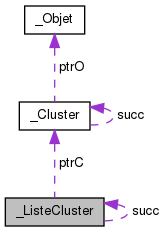
\includegraphics[scale=0.5]{images/struct_liste_cluster.png}
\caption{Graphe de collaboration de la structure ListeCluster}
\end{figure} 


\subsubsection{Cluster}

Ci-dessous la représentation de la structure Cluster. 
\begin{figure}[!h]
\texttt{Cluster = \^\,Place;}
\paragraph{}
 \texttt{ Place = enregistrement 
\begin{description}
\item ptrO : Objet;
\item succ : Cluster;
\item fin;
\end{description}
}
\caption{Représentation de la structure Cluster}
\end{figure}

\paragraph{}
La structure Cluster est une liste cha\^inée à l'aide de l'attribut "succ". Chaque cellule pointe vers une autre cellule de la structure et vers un élément de type Objet.
Ci-dessous, le graphe de collaboration de la structure Cluster.  

\begin{figure}[!h]
\center
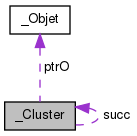
\includegraphics[scale=0.5]{images/struct_cluster.png}
\caption{Graphe de collaboration de la structure Cluster}
\end{figure} 

\subsubsection{Objet}

La structure Objet peut-\^etre représentée de la manière suivante : 
\begin{figure}[!h]
\texttt{Objet = \^\,Element;}
\paragraph{}
 \texttt{Element = enregistrement 
\begin{description}
\item idObjet : Entier non signé;
\item coordx : Entier;
\item coordy : Entire;
\item poids : Entier non signé;
\item trie : Bool
\item fin;
\end{description}
}
\caption{Représentation de la structure Objet}
\end{figure}

\paragraph{}
Un élément de la structure Objet représente un produit. Pour chaque produit, on indiquera : 
\begin{itemize}
\item[•]\textbf{l'identifiant} : idObjet
\item[•]\textbf{son coordonnée x} : coordx
\item[•]\textbf{son coordonnée y} : coordy 
\item[•]\textbf{son poids} : poids
\item[•]\textbf{s'il a déjà été trié} : trie
\end{itemize}


\subsection{Architecture}

\paragraph{}
Le programme est axé autour d'un fichier principal appelé par le \textit{main}, \textit{ClusterFirst.h}. Dans le \textit{main} sont aussi inclus les différentes structures citées auparavant(\ref{subsec:struct} page \pageref{subsec:struct}) ainsi que différents fichier de la librairie C. 
On peut représenter le graphe des dépendances par inclusion du \textit{main} de la façon suivante : 

\begin{figure}[!h]
	\center
	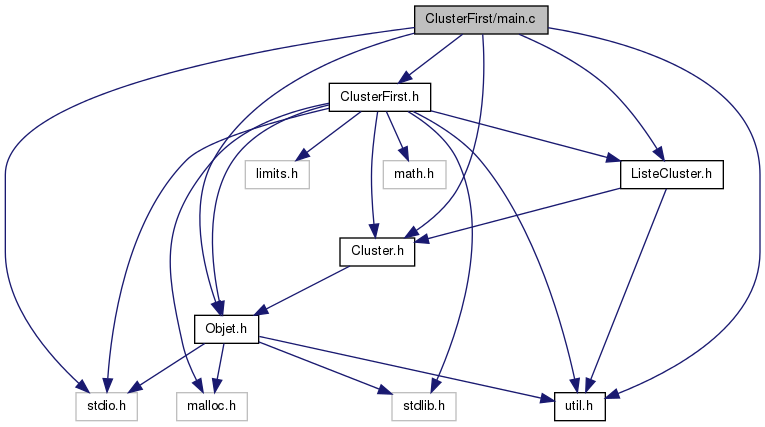
\includegraphics[scale=0.5]{images/main_inclusion.png}
	\caption{Graphe des dépendances par inclusion de \textit{main.c}}
\end{figure} 

\paragraph{}
Le main appel trois fonctions : 
\begin{itemize}
\item[•]\textbf{init} : Permet de récupérer les paramètres(capacité maximum du chariot ainsi que le fichier texte contenant les informations sur les produits, c'est à dire le carnet de commande) et affiche un message d'erreur si aucuns paramètres n'a été passé.
\item[•]\textbf{remplissageCluster}\footnote{cf algorithme n\degre \ref{algo:remplissageCluster}} : Découpe le carnet de commande en cluster.
\item[•]\textbf{trieListeCluster} \footnote{cf algorithme n\degre \ref{algo:trieListeCluster}}: Trie chaque cluster crée avec remplissageCluster pour que le chariot effectue l'itinéraire le plus court possible.
\end{itemize}

\paragraph{}
Le graphe d'appel du \textit{main} (ci-dessous), montre tous les appels de fonction effectuer à partir celui-ci à travers les trois fonctions citées précédemment.

\begin{figure}[!h]
	\center
	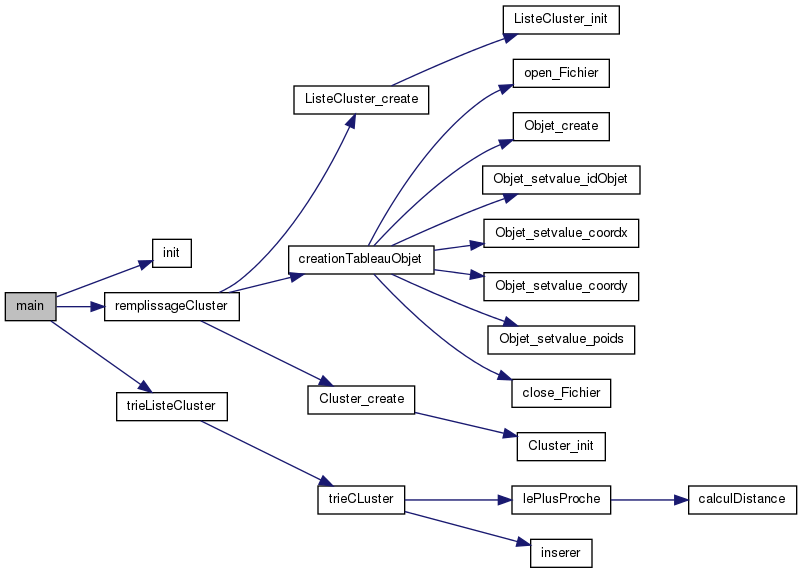
\includegraphics[scale=0.5]{images/main_appel.png}
	\caption{Graphe d'appel de la fonction \textit{main}}
\end{figure}

\section{Algorithmes}

\paragraph{}
Dans cette section, les principaux différents algorithmes seront décrits.

\subsection{Remplissage des clusters}

\paragraph{}
Afin de créer une liste de clusters, il faut tout d'abord remplir la structure Objet avec les informations des produits. Pour cela on va utiliser la fonction \textit{creationTableauObjet} dont voici l'algorithme : 

\begin{algorithm}[H]
\caption{Creation d'un tableau de pointeur vers des Objets : \textit{creationTabObjet}}
\label{algo:creationTabObjet}
\algsetup{indent=3em}
\begin{algorithmic}[1]
\REQUIRE { %
 entrées : $filename$ : fichier texte, $nb\_lignes$ : nombre de lignes, $cap\_max$ : capacité maximum du chariot}
\ENSURE { sortie : $tabObjet$ : le tableau de pointeur vers des Objets, $nb\_lignes$ : le nombre de produits}

\STATE $file \leftarrow ouvrirFichier(filename)$ 
\COMMENT{ouverture du fichier}
\STATE $allouer(tabObjet)$
\COMMENT{ allocation mémoire de $tabObjet$ }
\STATE $lire(file, nb\_lignes)$
\COMMENT{lecture de la première ligne et récupération du nombre d'item dans $nb\_lignes$}
\FOR[parcours du fichier ]{$indice$ \textbf{de} 1 \textbf{à} $nb\_lignes$ \textbf{faire}}
	\STATE $lire(file, idObjet, coordx, coordy, poids)$
	\COMMENT{lecture d'une ligne}
	\STATE $creer(Objet)$
	\COMMENT{allocation mémoire et initialisation de $Objet$}
	\STATE $Objet\uparrow idObjet \leftarrow idObjet$
	\STATE $Objet\uparrow coordx \leftarrow coordx$
	\STATE $Objet\uparrow coordy \leftarrow coordy$
	\STATE $Objet\uparrow poids \leftarrow poids$
	\IF[vérifie que le poids des produits est inférieur à la capacité du chariot]{($Objet\uparrow poids < cap\_max$)}
	\STATE $afficher($Erreur poids produits trop élévé$)$
	\STATE $exit$
	\ENDIF
	\STATE $tabObjet[indice] \leftarrow Objet$
\ENDFOR
\STATE $fermetureFichier(file)$
\COMMENT{fermeture du flux}
\RETURN $tabObjet$

\end{algorithmic}
\end{algorithm}

\paragraph{}
Après l'allocation de la structure Objet, on peut remplir les différents clusters à partir de la fonction \textit{remplissageCLuster}. L'algorithme de cette fonction est le suivant : 

\begin{algorithm}[H]
\caption{Remplissage des clusters : \textit{remplissageCluster}}
\label{algo:remplissageCluster}
\algsetup{indent=3em}
\begin{algorithmic}[1]
\REQUIRE { %
 entrées : $filename$ : fichier texte,$cap\_max$ : capacité maximum du chariot}
\ENSURE { sortie : $listeCluster$ : pointeur sur la tête de la liste de clusters}

\STATE $creer(listeCLuster)$ 
\COMMENT{allocation mémoire et création de $listeCluster$}
\STATE $tabObjet\leftarrow creationTabObjet(filename, nb\_lignes, cap\_max)$
\COMMENT{appel de la fonction $creationTabObjet$ }
\STATE $listeCLusterHead\leftarrow listeCluster$
\COMMENT{fait pointer la tête de liste vers $listeCluster$}
\FOR[Parcours de tabObjet ]{$indice$ \textbf{de} 1 \textbf{à} $nb\_lignes$ \textbf{faire}}
		\STATE $Objet \leftarrow tabObjet[indice]$	
		\COMMENT{$Objet$ reçoit le pointeur vers un Objet de la case $indice$ de $tabObjet$}
		\STATE $newCap \leftarrow listeCluster\uparrow cap + Objet\uparrow poids$
		\COMMENT{addition de la capacité du cluster en cours et du poids de l'objet a ajouter}
		\WHILE{(($cap\_max < newCap)\AND (listeCluster\uparrow succ \neq NULL$))}
			\STATE $listeCluster \leftarrow listeCluster\uparrow succ$
			\STATE $newCap \leftarrow listeCluster\uparrow cap + Objet\uparrow poids$
		\ENDWHILE
		\IF[s'il y a de la place pour ajouter l'objet]{$newCap \leq cap\_max$}
			\STATE $clusterTmp \leftarrow listeCluster\uparrow ptrC$
			\COMMENT{$clusterTmp$ pointe vers la tête de liste du cluster}
			\WHILE{($clusterTmp\uparrow succ \neq NULL$)} 
				\STATE $clusterTmp \leftarrow clusterTmp\uparrow succ$
				\COMMENT{parcours du cluster jusqu'à la fin}
			\ENDWHILE
			\STATE $creer(cluster)$
			\COMMENT{allocation mémoire et initialisation de $cluster$}
			\STATE $clusterTmp\uparrow succ \leftarrow cluster$
			\STATE $cluster\uparrow ptrO \leftarrow Objet$
			\STATE $listeCluster\uparrow cap \leftarrow newCap$
		\ELSE[si pas assez de place dans aucun cluster déjà existant]
			\STATE $creer(listeCLusterTmp)$
			\COMMENT{allocation mémoire et initialisation de $listeClusterTmp$}
			\STATE $listeCluster\uparrow succ \leftarrow listeClusterTmp$
			\STATE $listeCluster \leftarrow listeClusterTmp$
			\STATE $listeCluster\uparrow cap \leftarrow objet\uparrow poids$
			\STATE $creer(cluster)$
			\COMMENT{allocation mémoire et initialisation de $cluster$}
			\STATE $listecLuster\uparrow ptrC \leftarrow cluster$
			\STATE $cluster\uparrow ptrO \leftarrow objet$
		\ENDIF
		\IF{($listecluster\uparrow cap = cap\_max$)}
			\STATE $listeCLuster\uparrow fini \leftarrow TRUE$
		\ENDIF
\ENDFOR
\RETURN $listeClusterHead$


\end{algorithmic}
\end{algorithm}

\subsection{Trie des clusters}

\paragraph{}
Lorsque la liste des clusters est crée, il faut ensuite trier chacun d'eux pour que l'itinéraire du chariot soit le plus court possible. Pour ce faire, nous avons réaliser trois algorithmes :
\begin{enumerate}
\item\textit{trieListeCluster} \footnote{cf algorithme n\degre \ref{algo:trieListeCluster}} : Permet de trier la liste des Clusters
\item\textit{trieCluster}\footnote{cf algorithme n\degre \ref{algo:trieCluster}} : Trie chaque cluster
\item\textit{lePlusProche} \footnote{cf algorithme n\degre \ref{algo:lePlusProche}} : Cherche l'objet le plus proche de celui passer en paramètre dans son cluster
\end{enumerate}

\begin{algorithm}[H]
\caption{Trie de la liste des clusters : \textit{trieListeCluster}}
\label{algo:trieListeCluster}
\algsetup{indent=3em}
\begin{algorithmic}[1]
\REQUIRE { %
 entrées : $listeCluster$ : liste des clusters}
%\ENSURE { sortie : $listeCluster$ : pointeur sur la tête de la liste de clusters}

\WHILE{($listeCluster \neq NULL$)}
	\STATE $dist \leftarrow trieCluster(listeCluster\uparrow ptrC)$
	\COMMENT{retourne la distance à effectuer par le chariot dans le cluster}
	\STATE $listeCluster \leftarrow listeCluster\uparrow succ$
	\STATE $distTotal \leftarrow distTotal + dist$
\ENDWHILE
\STATE $afficher(la distance a parcourir par le chariot est : distTotal)$

\end{algorithmic}
\end{algorithm}

\begin{algorithm}[H]
\caption{Trie d'un cluster : \textit{trieCluster}}
\label{algo:trieCluster}
\algsetup{indent=3em}
\begin{algorithmic}[1]
\REQUIRE { %
 entrées : $head$ : pointeur vers la tête de la liste du cluster}
\ENSURE { sortie : $distTotal$ : distance à parcourir par le chariot dans le cluster}

\STATE $enCours \leftarrow head$
\WHILE{($enCours\uparrow succ \neq NULL$)}
	\STATE $comp++$
	\COMMENT{compte le nombre d'item du cluster}
\ENDWHILE
\STATE $enCours \leftarrow head$
\WHILE{($enCours \neq NULL$)}
	\STATE $clusterTmp \leftarrow lePlusProche(head, enCours, dist, compt)$
	\COMMENT{retourne le cluster le plus proche de enCours}
	\STATE $listeCluster \leftarrow listeCluster\uparrow succ$
	\STATE $distTotal \leftarrow distTotal + dist$
	\STATE $inserer(enCours, clusterTmp, head)$
	\COMMENT{insère la cellule clusterTmp avant celle d'enCours et refait le chainage de la liste}
	\STATE $enCours \leftarrow clusterTmp$
\ENDWHILE
\STATE $afficher(la distance a parcourir par le chariot est : distTotal)$
\RETURN $distTotal$

\end{algorithmic}
\end{algorithm}


\begin{algorithm}[H]
\caption{Cherche le cluster le plus proche : \textit{lePlusProche}}
\label{algo:lePlusProche}
\algsetup{indent=3em}
\begin{algorithmic}[1]
\REQUIRE { %
 entrées : $head$ : pointeur vers la tête de la liste du cluster, $enCours$ : pointeur vers le cluster courant, $distmin$ : distance minimum, $compt$ : nombre de cellule du cluster}
\ENSURE { sortie : $plusProche$ : cluster le plus proche de enCours, $distmin$ : distance entre $plusProche$ et $enCours$}

\STATE $ObjetCourant \leftarrow enCours\uparrow ptrO$
\STATE $minDist \leftarrow infini$
\STATE $cluster \leftarrow head$
\FOR[parcours du cluster]{$indice$ \textbf{de} 1 \textbf{à} $compt$ \textbf{faire}}
	\STATE $objetTmp \leftarrow cluster\uparrow ptrO$
	\IF[si $objetTmp$ n'a pas déjà été trié et s'il est différent de $objet$]{(($objetTmp\uparrow trie = FALSE) \AND (objetTmp \neq objet$))}
		\STATE $dist \leftarrow calculDistance(objet\uparrow coordx, objet\uparrow coordy, objetTmp\uparrow coordx, objetTmp\uparrow coordy)$
		\COMMENT{calcul la distance euclidienne entre $objetTmp$ et $objet$}
		\IF{($dist < minDist$)}
			\STATE $minDist \leftarrow dist$
			\STATE $plusProche \leftarrow cluster$
		\ENDIF
	\ENDIF
	\STATE $cluster \leftarrow cluster\uparrow succ$
\ENDFOR
\RETURN $plusProche$
\end{algorithmic}
\end{algorithm}

%%%%%%%%%%%%%%%%%%%% CHAPITRE 3 %%%%%%%%%%%%%%%%%%%%%%

\chapter{Root First Cluster Second}

\section{Architecture du programme}

\subsection{Structure de données}

\subsection{Architecture}

\section{Algorithmes}

\subsection{Trie des items}

\subsection{Découpage en clusters}


%%%%%%%%%%%%%%%%%%%%%%% CHAPITRE 4 %%%%%%%%%%%%%%%%%%

\chapter{Test des différents heuristiques}
\label{chap:test}
%%%%%%%%%%%%%%%%%%%% CONCLUSION %%%%%%%%%%%%%%%%%%%%%%

\chapter{Conclusion}

%\annexes

\end{document}

